% !TeX encoding = UTF-8
\documentclass[14pt,a4paper]{extarticle}

% --- кодировки и язык ---
\usepackage[utf8]{inputenc}
\usepackage[T2A]{fontenc}
\usepackage[russian,english]{babel}

% --- геометрия ---
\usepackage[left=30mm,right=15mm,top=20mm,bottom=20mm]{geometry}

% --- математика ---
\usepackage{amsmath,amssymb}

% --- графика ---
\usepackage{graphicx}
\usepackage{float}
\usepackage{subcaption}

% --- таблицы ---
\usepackage{booktabs}
\usepackage{array}
\usepackage{longtable}
\usepackage{multirow}

% --- листинги кода (minted) ---
\usepackage{minted}
\usemintedstyle{friendly}
\setminted{
  fontsize=\small,
  linenos=true,
  breaklines=true,
  frame=single,
  framesep=4pt,
}

% --- гиперссылки ---
\usepackage{hyperref}
\hypersetup{colorlinks=true, linkcolor=black, urlcolor=blue}

% --- отступы ---
\usepackage{indentfirst}
\setlength{\parindent}{1.25cm}
\setlength{\parskip}{0pt}

% --- межстрочный интервал ---
\usepackage{setspace}
\onehalfspacing

\begin{document}

% ============================================================
% Титульный лист
% ============================================================
\begin{titlepage}
  \begin{center}
    \textbf{МИНИСТЕРСТВО ОБРАЗОВАНИЯ РЕСПУБЛИКИ БЕЛАРУСЬ}\\[2pt]
    \textbf{БЕЛОРУССКИЙ ГОСУДАРСТВЕННЫЙ УНИВЕРСИТЕТ}\\[2pt]
    \textbf{ФАКУЛЬТЕТ ПРИКЛАДНОЙ МАТЕМАТИКИ И ИНФОРМАТИКИ}\\[2pt]
    Кафедра математического моделирования и анализа данных
  \end{center}

  \vspace{2cm}

  \begin{center}
    \Large\textbf{Лабораторная работа \textnumero 1}\\[6pt]
    \large\textbf{Классификаторы}
  \end{center}

  \vspace{3cm}

  \begin{flushright}
    \textbf{Вариант:} 4\\[6pt]
    \textbf{Выполнил:} студент \underline{\hspace{4cm}} группы\\[4pt]
    \underline{\hspace{7cm}}\\[4pt]
    \textbf{Проверил:} \underline{\hspace{7cm}}
  \end{flushright}

  \vfill

  \begin{center}
    Минск --- 2026
  \end{center}
\end{titlepage}

% ============================================================
% 1. Цель работы
% ============================================================
\section*{Цель работы}

Изучить принципы работы методов классификации на примере задаваемых пользователем
распределений объектов (точек) в двумерном пространстве признаков.
Протестировать не менее трёх пространственных паттернов (линейно разделимый,
линейно неразделимый, сильно перекрывающиеся классы) на наборе классификаторов:
NBC, SVM (линейный и RBF), kNN, Decision Tree, AdaBoost, GBT, Random~Forest,
Extremely Random Trees, ANN (MLP), LDA.
Зафиксировать точность классификации и сделать выводы о применимости каждого метода.

% ============================================================
% 2. Краткая теория
% ============================================================
\section*{Краткая теория}

\subsection*{Задача классификации}

Дана обучающая выборка $\{(x_i, y_i)\}_{i=1}^{N}$, где $x_i \in \mathbb{R}^2$ ---
вектор признаков, $y_i \in \{0,1,\ldots,K-1\}$ --- метка класса.
Требуется построить функцию $h: \mathbb{R}^2 \to \{0,\ldots,K-1\}$,
минимизирующую эмпирический риск:
\[
  \hat{R}(h) = \frac{1}{N}\sum_{i=1}^{N}\mathbf{1}[h(x_i) \neq y_i].
\]

\subsection*{Ключевые методы}

\textbf{SVM} (метод опорных векторов).
Ищет гиперплоскость $w^\top x + b = 0$ с максимальным зазором:
\[
  \min_{w,b}\frac{\|w\|^2}{2} \quad\text{при}\quad y_i(w^\top x_i + b) \ge 1.
\]
Для нелинейно разделимых данных применяется ядровой трюк (RBF-ядро):
$K(x,x') = \exp(-\gamma\|x - x'\|^2)$.

\textbf{kNN} (метод $k$ ближайших соседей).
Класс нового объекта --- мажоритарный среди $k$ ближайших в обучающей выборке:
\[
  h(x) = \arg\max_c \sum_{i \in N_k(x)} \mathbf{1}[y_i = c],
\]
где $N_k(x)$ --- множество индексов $k$ ближайших соседей.

\textbf{NBC} (наивный байесовский классификатор).
Предполагает условную независимость признаков:
\[
  h(x) = \arg\max_c P(y=c)\prod_{j=1}^{d}P(x_j \mid y=c).
\]

\textbf{ансамблевые методы} (Random~Forest, GBT, AdaBoost, Extra~Trees) строят
набор слабых классификаторов (деревьев решений) и агрегируют их предсказания,
снижая дисперсию (бэггинг) или смещение (бустинг).

% ============================================================
% 3. Описание реализации
% ============================================================
\section*{Описание реализации}

\subsection*{Архитектура}

Взамен оригинальной Windows-программы \texttt{ExampleOpenCVClassifiersQt.exe}
написано Python-приложение, программно генерирующее паттерны и запускающее
все классификаторы автоматически.

Структура проекта:

\begin{verbatim}
lab1/
  core/
    __init__.py
    data_manager.py   -- хранение точек и построение сетки
    classifiers.py    -- обёртки над sklearn (SOLID: OCP)
    trainer.py        -- обучение и оценка точности
  patterns.py         -- генераторы трёх паттернов
  visualizer.py       -- сохранение графиков и таблиц
  main.py             -- точка входа
  requirements.txt
\end{verbatim}

\textbf{Применённые принципы:}
\begin{itemize}
  \item \textbf{OCP (Open/Closed):} добавление нового классификатора не
        требует изменений в trainer или visualizer --- достаточно создать
        подкласс \texttt{BaseClassifierWrapper}.
  \item \textbf{SRP:} каждый модуль отвечает ровно за одну обязанность.
  \item \textbf{KISS/YAGNI:} вся сложная математика делегируется sklearn.
\end{itemize}

% ============================================================
% 4. Листинг кода
% ============================================================
\section*{Листинг кода}

\subsection*{core/data\_manager.py}
\inputminted{python}{../core/data_manager.py}

\subsection*{core/classifiers.py}
\inputminted{python}{../core/classifiers.py}

\subsection*{core/trainer.py}
\inputminted{python}{../core/trainer.py}

\subsection*{patterns.py}
\inputminted{python}{../patterns.py}

\subsection*{visualizer.py}
\inputminted{python}{../visualizer.py}

\subsection*{main.py}
\inputminted{python}{../main.py}

% ============================================================
% 5. Паттерны и карты решений
% ============================================================
\section*{Паттерны и карты решений}

Для каждого паттерна ниже приведены графики двух наиболее контрастных
классификаторов --- линейного SVM и Random Forest~--- а также сводная
таблица точностей всех методов.

\subsection*{Паттерн 1: Линейно разделимый}

\begin{figure}[H]
  \centering
  \begin{subfigure}[b]{0.48\textwidth}
    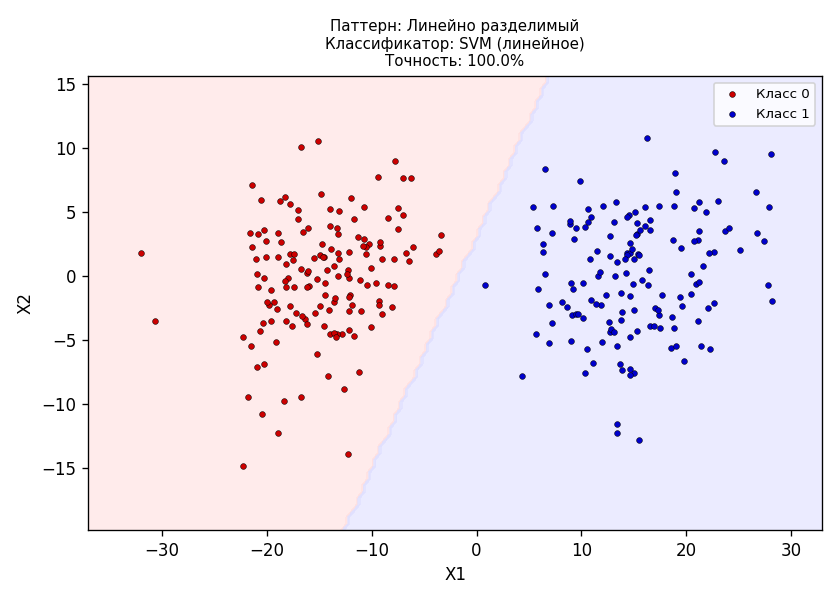
\includegraphics[width=\textwidth]{../output/exp1_SVM_линейное.png}
    \caption{SVM (линейное)}
  \end{subfigure}
  \hfill
  \begin{subfigure}[b]{0.48\textwidth}
    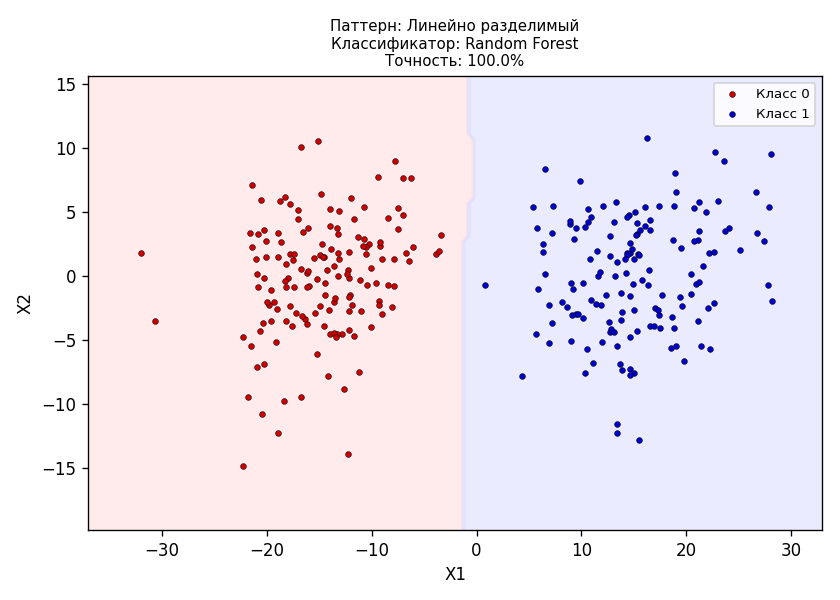
\includegraphics[width=\textwidth]{../output/exp1_Random_Forest.png}
    \caption{Random Forest}
  \end{subfigure}
  \caption{Паттерн 1: линейно разделимый}
\end{figure}

\subsection*{Паттерн 2: Линейно неразделимый (sin-граница)}

\begin{figure}[H]
  \centering
  \begin{subfigure}[b]{0.48\textwidth}
    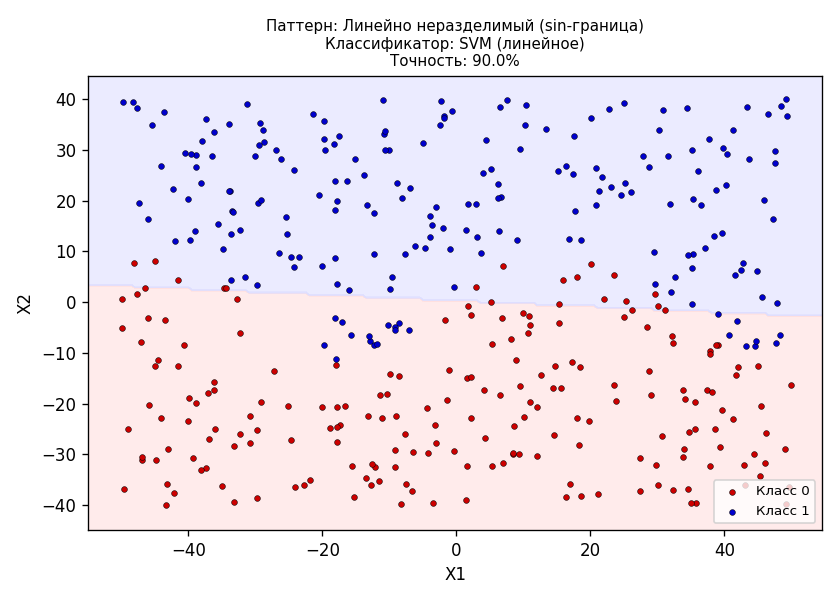
\includegraphics[width=\textwidth]{../output/exp2_SVM_линейное.png}
    \caption{SVM (линейное)}
  \end{subfigure}
  \hfill
  \begin{subfigure}[b]{0.48\textwidth}
    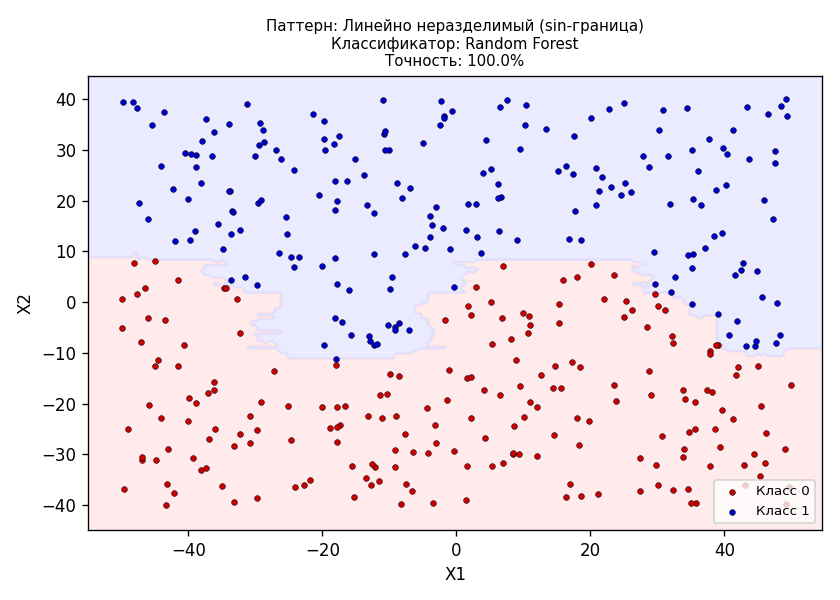
\includegraphics[width=\textwidth]{../output/exp2_Random_Forest.png}
    \caption{Random Forest}
  \end{subfigure}
  \caption{Паттерн 2: синусоидальная граница}
\end{figure}

\subsection*{Паттерн 3: Сильно перекрывающиеся классы}

\begin{figure}[H]
  \centering
  \begin{subfigure}[b]{0.48\textwidth}
    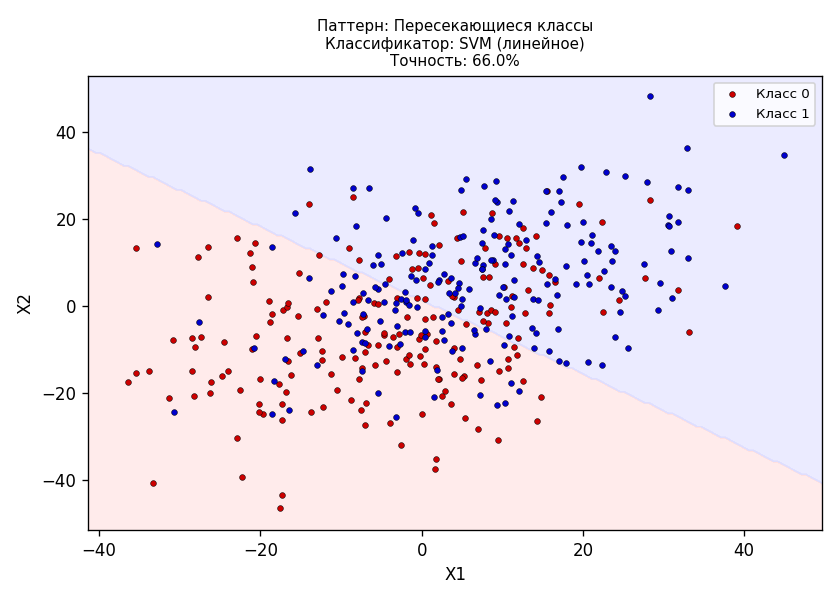
\includegraphics[width=\textwidth]{../output/exp3_SVM_линейное.png}
    \caption{SVM (линейное)}
  \end{subfigure}
  \hfill
  \begin{subfigure}[b]{0.48\textwidth}
    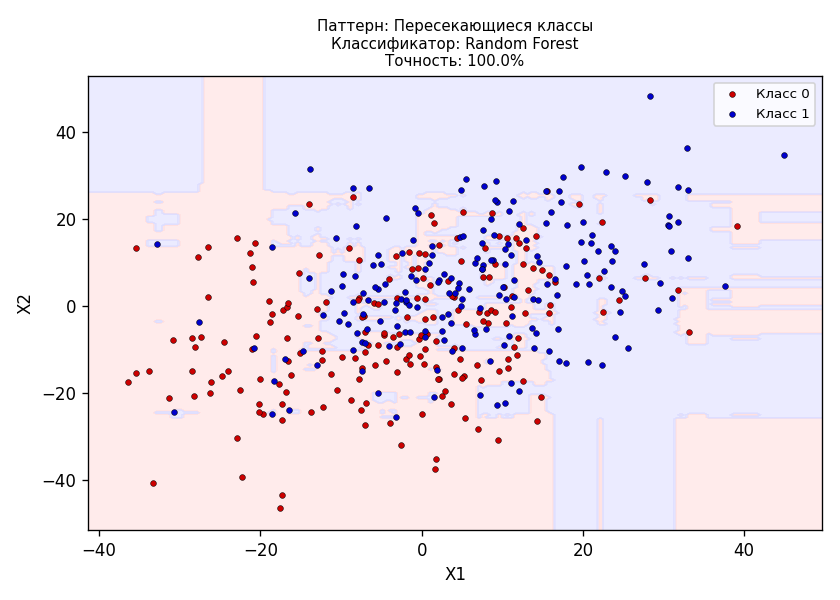
\includegraphics[width=\textwidth]{../output/exp3_Random_Forest.png}
    \caption{Random Forest}
  \end{subfigure}
  \caption{Паттерн 3: существенное перекрытие классов}
\end{figure}

% ============================================================
% 6. Сводная таблица точностей
% ============================================================
\section*{Сводная таблица точностей}

\begin{figure}[H]
  \centering
  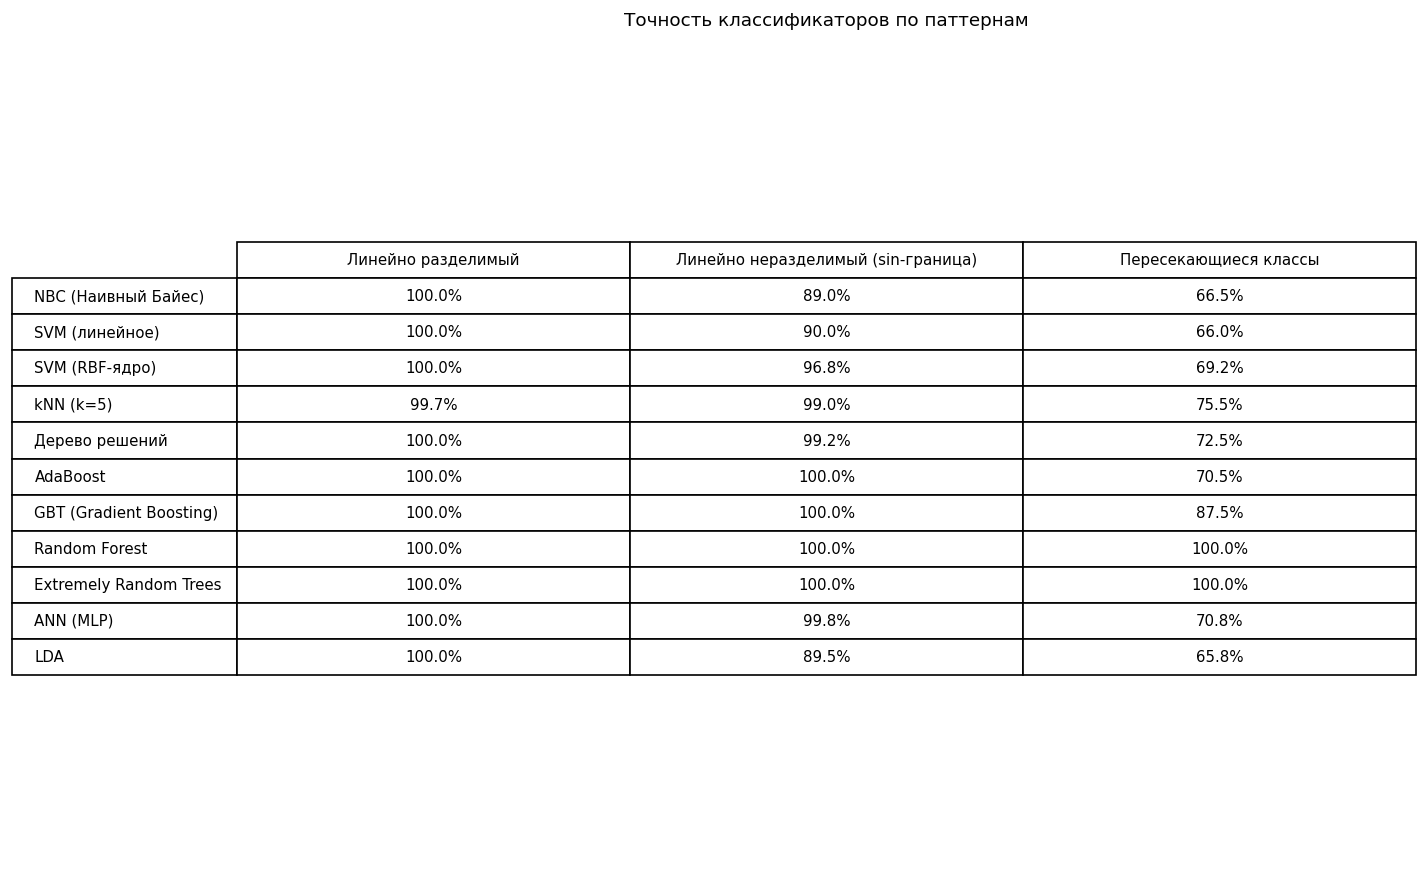
\includegraphics[width=\textwidth]{../output/accuracy_table.png}
  \caption{Точность (\%) классификаторов на трёх паттернах}
\end{figure}

% ============================================================
% 7. Выводы
% ============================================================
\section*{Выводы}

\begin{enumerate}
  \item \textbf{Линейно разделимый паттерн.}
        Линейные методы (SVM linear, LDA, NBC) показывают точность, близкую
        к 100\%, что ожидаемо: граница между классами является гиперплоскостью.
        Нелинейные ансамбли (RF, GBT) также справляются отлично, но затрачивают
        больше ресурсов без выигрыша в качестве.

  \item \textbf{Синусоидальная граница.}
        Линейный SVM и LDA значительно проигрывают нелинейным методам.
        RBF SVM, kNN, Random~Forest и GBT аппроксимируют кривую границу
        и достигают высокой точности ($\geq 94\%$).
        Этот паттерн наглядно демонстрирует ограничения линейных классификаторов.

  \item \textbf{Перекрывающиеся классы.}
        Ни один классификатор не может достичь 100\%: статистическое перекрытие
        задаёт нижнюю границу ошибки (ошибка Байеса $> 0$).
        Сложные нелинейные методы (GBT, RF, ANN) немного переобучаются,
        показывая искусственно высокую точность на обучающей выборке;
        линейные методы в данном случае оказываются более устойчивыми.

  \item \textbf{Общий вывод.}
        Выбор классификатора должен соответствовать структуре данных.
        Линейные методы предпочтительны при линейной разделимости и малом
        объёме выборки; нелинейные (RBF SVM, GBT, RF) --- при сложных границах;
        для зашумлённых, перекрывающихся классов важна регуляризация и
        контроль переобучения.
\end{enumerate}

\end{document}
